% Chapter Template

\chapter{Methods} % Main chapter title

\label{Chapter 2} % Change X to a consecutive number; for referencing this chapter elsewhere, use \ref{ChapterX}


%-----------------------------------
%	SECTION 1
%-----------------------------------
\section{Dietary diary collected in the NDNS RP}\vspace{-0.3cm}

Participants were asked to keep a record of everything eaten or drunk over four consecutive days. Interviewers undertook three visits with each participant. At the first visit, the interviewer explained the method followed a protocol, taking participants through the sections in the diary including how to describe details of food and drink and portion size and an example day. The second was a brief visit to check for compliance, answer questions or deal with problems and review the diary to identify and edit possible omissions and missing detail. The third visit was to collect the diary and again review and edit possible omissions. 

In the diary, participants were asked to record portion sizes in household measures (e.g. one tablespoon of beans, one Kit Kat finger-size), or for packaged foods to note the weight indicated on the packet. For homemade dishes, participants were asked to record on a separate page in the diary the individual ingredients and quantities for the whole dish along with a brief description of the cooking method and how much of dish they had consumed. For each eating occasion, in addition to the details of what and how much was eaten, participants were also asked to record: when was it, where they were, and who they were eating with. An example, used as guidance for participants, of a food diary for one day is shown in \textbf{Appendix \ref{AppendixE}}.\vspace{-0.3cm}

\subsection{Definition of carbohydrate intake}\vspace{-0.3cm}

Detailed dairy checking was performed to code and convert the food consumption into energy and nutrients intake. Intakes of nutrients were calculated from the food consumption records using a specially adapted Nutrient Databank \parencite{smithers1993maff}, which was originally developed by the Ministry of Agriculture, Fisheries, and Food (MAFF) for the Dietary and Nutritional Survey of British Adults. Further details of data
coding and editing are outlined in Appendix A of the NDNS official reports \parencite{NDNSofficial}. Specifically, the main variables that we adopted in the current analysis were defined as: 

\begin{itemize}
	\item Total energy intake = (protein $\times$ 17) + (fat $\times$ 37) + (carbohydrate $\times$ 16) + (alcohol $\times$ 29)  kJ;
	\item Carbohydrate intake = total sugars + starch; 
	\item Where all quantities above were measured as mass in grams.
\end{itemize}

Time across a typical survey day was divided into 7 time slots in the dietary diary of NDNS RP: 6 am to 9 am, 9 am to 12 noon, 12 noon to 2 pm, 2 pm to 5 pm, 5 pm to 8 pm, 8 pm to 10 pm, and 10 pm to 6 am next morning. To produce a list of discrete responses for our variable of interest, the energy consumed within each time slot over the four days of survey for each participant were calculated. The percentages of total energy intake contributed by carbohydrate within each time slot were then calculated. Since we planned to apply latent class analysis (LCA) in the current study, in which the observed indicators for latent classes must be categorical, the responses were then dichotomised according to these percentages of the energy intake at a cut-off value of 50\%, i.e. if within a time slot where there any energy intake occurred, carbohydrate consumption was categorised by whether its energy contribution was lower or higher/equal to 50\% of total energy intake within that time slot. Consequently, for each day of the recording, there were 7 data points generated by the diary. Each data point included one of the following responses:

\begin{itemize}
	\item Not eating any food (energy intake = 0 kJ); 
	\item Eating, and carbohydrate contributed less than 50\% of the total energy intake;
	\item Eating, and carbohydrate contributed higher or equal to 50\% of the total energy intake.
\end{itemize}
\vspace{-0.5cm}


%----------------------------------------------------------------------------------------
%	SECTION 2
%----------------------------------------------------------------------------------------

\section{Survey Data}\vspace{-0.3cm}

%-----------------------------------
%	SUBSECTION 1
%-----------------------------------
\subsection{Survey selection method}\vspace{-0.3cm}

The NDNS RP participants were drawn from the UK Postcode Address File, a list of all the addresses in the UK. The addresses were clustered into Primary Sampling Units (PSUs), small geographical areas, based on postcode sectors, randomly selected from across the UK. A list of 27 or 28 addresses was then randomly selected from each PSU.

Overall, for years 1 to 8 combined, a sample of 39,300 addresses was selected from 1,438 PSUs. The sampling selection process was: 

\begin{itemize}
	\item Randomly select PSUs from the Postcode Address File; 
	\item Randomly select 27 or 28 addresses in that postcode area; 
	\item Randomly select one household at that address for interviews; 
	\item Selected addresses where children resided were randomly allocated to one of two groups to determine whether an adult (aged 19 years or older) and a child (aged 1.5 to 18 years) or a child only, were selected for interviews.
\end{itemize}
\vspace{-0.6cm}
%-----------------------------------
%	SUBSECTION 2
%-----------------------------------
\subsection{Response rates}\vspace{-0.3cm}

The response rates for completion of the dietary diary (three or four days) were 56\%, 53\%, 53\%, for years 1 to 4, 5 to 6, and 7 to 8, respectively. A total of 6,155 adults aged 19 years and older were kept in the current study. 
\vspace{-0.6cm}

\subsection{Strata and weightings}\vspace{-0.3cm}

It is necessary to apply weighting factors to the data collected in the NDNS RP for two reasons: to remove any bias in the observed results which may be due to differences in the probability of households and individuals being selected to take part; and to attempt to reduce differential non-response bias by age, sex, and geographical region. 

The strata used to calibrate proportions in the sample include: age-group (1.5-3, 4-6, 7-10, 11-15, 16-18, 19-24, 25-29, 30-39, 40-49, 50-59, 60-64, 65-69, and over 70 years); sex (men or women); and regions (Northern Ireland, Scotland, Wales, and the nine regions of England). 

Two steps of the weighting system were designed in the NDNS RP to assure that the combined sample would be representative of the UK population: 

\begin{enumerate}
	\item An overall selection weight, which is the product of the address, dwelling unit, catering (household) unit, and individual selection weights, was generated to correct for the unequal selection probabilities. These weights are the inverses of the selection probabilities at each level of the random sampling process, and they can be used to compensate for differences in the chance of selection of an individual.
	\item An iterative procedure was used to adjust the selection weights until the distribution of the weighted sample matched that of the population for age-group, sex, and geographical region. Population distributions were taken from the mid-year population estimates \parencite{OfficeofNationalStat}. 
\end{enumerate}


Another two sets of weights were generated to correct for differential non-response (either due to refusal or inability) to 1) nurse visit and 2) giving a blood sample. Response rates to the nurse visit among those completed a dietary diary was approximately 75\%, to the blood sample in adults were 51\%, 57\%, and 50\% for years 1 to 4, 5 to 6, and 7 to 8, respectively. In creating the nurse/blood sample weight, a logistic regression model was used by the NDNS RP study team to model the relationship between response to nurse visit/giving a blood sample and a set of predictor variables (socio-demographic, participant and catering/household unit characteristics). The model generated a predicted probability for each participant, which is the probability would agree to a nurse visit/provide a blood sample, given the characteristics of the individual and the household unit. Participants with characteristics associated with non-response were under-represented in the sample and therefore receive a low predicted probability. The inverses of these predicted probabilities were used as a set of non-response weights so that participants with a low predicted probability got a larger weight, increasing their representation in the sample. Then the nurse/blood sample weights were re-scaled so that the sum of the weights equalled the number of participants who had a nurse visit or who provided a blood sample. The final nurse/blood weights should, therefore, make the sample participants representative of all eligible persons in the population. 

Further details of the weighting system developed by the NDNS RP are described in Appendix B of the reports published by Public Health England (PHE) \parencite{bates2014national,roberts2018national,NDNSofficial}.\vspace{-0.6cm}

\subsection{Socio-demographic status, lifestyle, physical activity, anthropometric measurements and biochemical analyses}\vspace{-0.3cm}

Computer-assisted personal interviews were conducted for the selected individuals by trained interviewers to collect background information on smoking habits (current, ex-smokers, and never), ethnicity (white, non-white), education level (lower than degree/degree or above level), living with a partner or not, and other socio-demographic variables. Participants also had their height, weight, blood pressure, and waist circumferences (WC) measured by the nurses. 

Specifically, blood pressure was measured in a sitting position using an automated, validated machine, the Omron HEM907, after a five-minute rest. The mean of the second and third readings, taken at one-minute intervals, were used in the current report. Hypertension was defined as with systolic blood pressure of 140 mmHg or above, and/or diastolic blood pressure of 90 mmHg or above, and/or taking any medication specifically to reduce blood pressure. 

A self-completion questionnaire - the Recent Physical Activity Questionnaire  \parencite{besson2009estimating} (RPAQ, developed by the MRC Epidemiology Unit Cambridge) was used to estimate physical activity from year 2 of the survey. The RPAQ was designed to assess usual physical activity in the last month in four domains: home, work, commuting to work, and leisure activities. Detailed descriptions of the assessment of adult physical activity in the NDNS RP and the processing of data are available in Appendices G and V of the published reports \parencite{bates2014national,roberts2018national,NDNSofficial}. 

Blood samples were stored at 4 $^\circ$C, and sent directly by post to the Department of Haematology and Department of Clinical Biochemistry and Immunology, Addenbrooke's Hospital, Cambridge within two hours of their collection. Serum samples were obtained by centrifugation of the coagulated blood sample. Serum total, High-Density Lipoprotein (HDL) and Low-Density Lipoprotein (LDL) cholesterol, triglycerides (TG), fasting blood glucose, haemoglobin A1C were measured. A1C value of 6.5\% was used as the cut off point for diagnosing diabetes.

Body mass index (BMI) was calculated as weight in kilograms divided by height in square meters. BMI was then categorised into less than 25 kg/m\textsuperscript{2} (normal weight), 25 to 30 kg/m\textsuperscript{2} (overweight), and higher or equal to 30 kg/m\textsuperscript{2} (obese). 

\subsection{Ethical approval}\vspace{-0.3cm}

Ethical approval for the survey was obtained from the Oxfordshire A Research Ethics Committee. The letters of approval for the original submission and subsequent substantial amendments, together with approved documents, were sent to all Local Research Ethics Committees covering areas where fieldwork was being conducted. Research governance approval was sought for all participating NHS laboratories and obtained where required by the Research and Development Committee for each laboratory. Ethical approval for the current project was obtained from the MSc Research Ethics Committee of the London School of Hygiene \& Tropical Medicine (LSHTM MSc Ethics Ref: 15624). 


%-----------------------------------
%	SECTION 2
%-----------------------------------
\section[Statistical methods]{Statistical methods}

\subsection{Latent Class Analysis (LCA)}\vspace{-0.3cm}

Latent class analysis is a statistical technique that identifies categorical latent (unobserved) class variables on the basis of observed categorical variables \parencite{collins2010latent}. It belongs to the family of latent variable models and is directly analogous to the factor analysis model. The major difference is that the latent variable in LCA is categorical, not continuous as in factor analysis. The basic assumptions in LCA are independent observations and local independence, the latter as shown in the fundamental expression of a typical LCA model: \vspace{-0.8cm}

\begin{equation}
P(U_{i1} = s_1, U_{i2} = s_2, \cdots, U_{ik} = s_k) = \sum_{t=t}^{T}P(C_i = t)\prod_{k = 1}^{K}P(\mathbf{U_{ik}} = \mathbf{s_k} | C_i = t)
\label{LCA}
\end{equation}\vspace{-0.7cm}

Where, 

\begin{itemize}
	\item $P(U_{i1} = s_1, U_{i2} = s_2, \cdots, U_{ik} = s_k)$ is the probability of observing a particular vector of responses for $i$th observation;
	\item $P(C_i = t)$ is the probability that a randomly selected $i$th observation will be in class $t$;
	\item $P(\mathbf{U_{ik}} = \mathbf{s_k} | C_i = t)$ is the probability of a particular observed response pattern $\mathbf{U_{ik}} = \mathbf{s_k}$ conditional on membership in latent class $t$.
\end{itemize}


\textbf{Equation \ref{LCA}} indicates that responses for an observation to the measuring variables are independent of one another given its membership in latent class $t$. However, in the NDNS RP data set, the assumption of independent observations is violated. Each individual completed their dietary diary for three/four consecutive days, their diary recordings were later converted into three/four vectors of categorical responses reflecting the type of carbohydrate consumption at each time slot of the day. The observed sequences (observed days) are nested within the participants and therefore are not independent. This nested data structure requires multilevel techniques. 
\vspace{-0.3cm}

%-----------------------------------
%	SUBSECTION 2
%-----------------------------------

\subsection{Multilevel Latent Class Analysis (MLCA)}\vspace{-0.3cm}


Multilevel latent class analysis accounts for the nested structure of the data by allowing latent class intercepts to vary across level 2 units, thereby examining if and how level 2 units influence the level 1 latent classes. These random intercepts allow the probability of membership in a particular level 1 (observation days) latent class to vary across level 2 units (e.g., here in the current context are the individuals). Essentially this allows the probability that an observation day will belong to a
particular day-level latent class to vary across individual-levels.\vspace{-0.5cm}

\subsubsection{Parametric approach}\vspace{-0.3cm}

Proposed by Vermunt \parencite{Vermunt, vermunt2008latent} and Asparouhov and Muth\'en \parencite{muthen2009multilevel},  a traditional, parametric approach can be applied using a logistic regression model. For example, let's assume that there are two types of observation days in the dietary survey--high and low carbohydrate eating days. In an unconditional logistic regression model, the probability of the outcome (i.e. an observed high carbohydrate eating day vs. a low carbohydrate eating day) is constant within the individual-level, which means for each person throughout his/her survey there is some probability of following a high carbohydrate eating day. A random effect considers the individuals (level 2) to be drawn from the adult population in the UK, and the probability of the outcome (i.e. high carbohydrate eating days) across individuals is considered to be a random variable \parencite{snijders2011multilevel}. 

Thus, for a binary outcome $C_{ij} = 0, 1$ (low $=0$ or high $=1$ carbohydrate eating days), where $i$ denotes the observation days $(i = 1, 2, 3, 4)$, and $j$ denotes the individual $(j = 1, 2, \cdots, 6155)$, the 2-level random intercept logistic regression model can be expressed as:\vspace{-0.4cm}


\begin{equation}
\begin{aligned}
\text{logit}[P(C_{ij} = 1)] & = \beta_{0j} + \beta_{1}x_{ij} \;\;\;\;\;\;\;\;\; \textbf{(day-level)}  \\
\beta_{0j} & = \gamma_0 + \gamma_1 w_j + u_{0j} \; \textbf{(individual-level)} \\ 
\Rightarrow P(C_{ij} = 1) & = \frac{\exp{(\gamma_0 + \beta_{1}x_{ij} + \gamma_1 w_j + u_{0j})}}{1 + \exp{(\gamma_0 + \beta_{1}x_{ij} + \gamma_1 w_j + u_{0j})}} \\
\end{aligned}
\label{randomLCA}
\end{equation}
\vspace{-0.3cm}

Where we define: 

\begin{itemize}
	\item $\text{logit}{(x)} = \log{\frac{x}{1-x}}$, where $x \in [0,1]$;
	\item $P(C_{ij} = 1)$ as the probability that the randomly selected $i$th observation day of the $j$th individual is a high carbohydrate eating day;
	\item $\beta_{0j}$ as the random intercept, for the outcome $C_{ij} = 1$; 
	\item the random deviation of the individuals $u_{0j}$ are assumed be normally distributed (i.e. $u_{0j} \sim N(0, \sigma_{u_0}^2)$), the magnitude of the $u_{0j}$ variance ($\sigma_{u_0}^2$) indicates the influence of the individuals (level 2);
	\item $x_{ij}, w_j$ is the predictors for day-level (weekdays or weekends) and individual-level, such as age, and sex.
\end{itemize}



The same framework can be used to consider random effects in an LCA model, but instead of saying that $C_{ij}$ is either low or high carbohydrate eating days as if we already know the set of latent classes, it is now replaced by a latent variable $G_{ij}$ which indicates the typologies of carbohydrate eating patterns. Then we can use the day-level data to assess the log-odds of belonging to the $k$th type of carbohydrate eating pattern on a specific day of the survey and allow the log-odds to vary across individuals. Therefore, for some persons, the log-odds of having a $k$th type of carbohydrate eating pattern during the survey can be high, but for the other persons, the log-odds of following the $k$th type of carbohydrate eating pattern can be low. 

If the day-level LCA model (carbohydrate eating temporal pattern typologies) is best defined by $T (T \geqslant 2)$ latent classes, then $T-1$ random intercept will be specified by a two-level multinomial logistic regression model. Similar to the typical LCA models, the latent class variable in a MLCA is defined by multiple observed indicators (here is defined by the responses of eating carbohydrate within each time slots, throughout three/four consecutive days of their survey period). Considering the latent class indicators are indicator variables ($U_{ijk}$), the MLCA model can be written as follows:\vspace{-1cm}

\begin{equation}
%\begin{aligned}
P(U_{ij1} = s_1, U_{ij2} = s_2, \cdots, U_{ijk} = s_{k}) = \sum_{t=1}^{T}P(G_{ij}=t)\prod_{k=1}^{K}P(U_{ijk} = s_k | G_{ij} = t)
%\end{aligned}
\label{MLCA}
\end{equation}
\vspace{-0.8cm}


Where, 

\begin{itemize}
	\item $ U_{ijk} $ represents the response of carbohydrate eating (one of the following: not eating any food, $< 50\%$ of the energy, or $\geqslant 50\%$ of the energy) on the $i$th day of the survey ($i \in (1,2,3,4)$) in $j$th individual at the $k$th time slot of the day ($k \in (1, 2, 3, \cdots, 7)$);
	\item $G_{ij}$ denotes the latent class membership for $j$th individuals on the $i$th day of the survey, the total number of day-level latent class is $T$;
%	\item A specific latent class is referred to as $t$, and the total number of level 1 latent classes is denoted by $T$;
	\item $P(U_{ijk} = s_k|C_{ij} = t)$ is the probability of a specific response pattern, conditional on membership in latent class $t$.
\end{itemize}


The $P(G_{ij} = t)$ in equation \ref{MLCA} is what we have already defined in equation \ref{randomLCA}: \vspace{-0.3cm} 

\begin{equation}
P(G_{ij} = t) = \frac{\exp{(\gamma_0 + \beta_{1}x_{ij} + \gamma_1 w_j + u_{0j})}}{1 + \exp{(\gamma_0 + \beta_{1}x_{ij} + \gamma_1 w_j + u_{0j})}} 
\end{equation}

\vspace{-0.5cm}
\subsubsection{Non-Parametric approach}\vspace{-0.3cm}


Since the parametric approach discussed above can be extremely computationally demanding \parencite{van2008using, vermunt2008latent}, an alternative approach is using a non-parametric MLCA \parencite{davidian2008growth}. In this approach, separate latent class models are specified for level 1 (observation days) and level 2 (individuals). Similar with the parametric MLCA approach, there are $T-1$ random intercepts, where $T$ is the number of level 1 latent classes. However, rather than assuming the random intercepts following a normal distribution, the non-parametric MLCA assumes a multinomial (discrete) distribution of the level 2 latent classes. This approach is less computationally demanding compared with the parametric approach. These level 2 (individual) latent classes reflect differences in the probability of belonging to a specific day-level latent class, so that individuals that have observation days with similar probabilities for the level 1 latent classes will be grouped together. The non-parametric MLCA model can be defined as follows: 

\begin{equation}
P(C_{ij} = t | CB_j = m)  = \frac{\exp(\gamma_{tm})}{\sum_{r=1}^{T}\exp(\gamma_{rm})}
\end{equation}

Where, 

\begin{itemize}
	\item $CB_j$ is the individual-level latent class membership for the $j$th individual;
	\item $\gamma_{tm}$ is the day-level and individual-level indicators. 
\end{itemize}

According to Finch and French's simulation study \parencite{finch2014multilevel}, non-parametric approach generally resulted in more accurate recovery of the underlying latent structure of the data at both levels and provided better latent class model compared with parametric approach. In the current project, we are interested in exploring both meaningful individual (level 2) latent classes and the daily (level 1) carbohydrate consumption classification. Therefore, non-parametric MLCA was employed 1) to identify latent classes of observation days (level 1) based on the subjects' responses to the 4-day food and drink diary and 2) to form distinct latent classes of individuals (level 2) based on the distribution of day-level carbohydrate eating temporal latent classes within individuals.\vspace{-0.3cm}
 

\subsection{Strategy of conducting MLCA}\vspace{-0.3cm}

To identify the best-fitting model, we used the following sequential modelling strategy \parencite{henry2010multilevel}: 

\begin{itemize}
	\item First, we ignored the multilevel structure of the data and estimated a series of traditional LC models to determine the number of classes at the observational day-level;
	\item Next, a series of MLCA models were fitted to account for the multilevel structure of the data. In these models, the number of day-level classes was based on the best fitting LCA model from the first step, and the LCA model at the individual-level was estimated to identify the number of individual-level latent classes;
	\item Last, once the number of individual-level latent classes was defined based on the previous stage, the number of day-level classes was modified (one class lower and one class higher than in the second step) to investigate the effect of changing level 1 classes and to confirm the best fitting model.
\end{itemize}

The number of classes in level 1 was determined by 1) the evaluation of model fit indices, including the Bayesian information criterion (BIC) and entropy, which is a statistic that summarizes latent class probabilities where values near 1 indicate better latent class separation; 2) the Lo-Mendell-Rubin Likelihood Ratio Test (LMR-LRT) \parencite{lo2001testing, nylund2007deciding} which compares $q$ vs. $q-1$ classes models, where $q$ is the number of latent classes; most importantly, 3) pattern interpretability. In the steps of performing multilevel LCA, where LMR-LRT is not available, the same rules of model fit indices and pattern interpretability were used to determine the optimal combination of latent classes in observation day-level and individual-level. MLCA models were fitted in Mplus 7.4 \parencite{muthen2005mplus}, the Mplus syntax and outputs are shown in \textbf{Appendix \ref{AppendixB}}. \vspace{-0.3cm}



%\section{Latent Class Growth Analysis (LCGA)}\vspace{-0.3cm}
%
%%LCGA is a statistical approach that models patterns in longitudinal data by classifying individuals into unobserved latent classes with more homogeneous patterns. LCGA is a special type of Growth Mixture Models (GMM), in which the variance of latent slope and intercept are fixed to zero within class, and allowed to vary only across classes. LCGA assumes that all individual growth trajectories within classes are homogeneous. 
%
%
%LCGA is a semi‐parametric technique used to identify distinct subgroups of individuals following a similar pattern of change over time on a given variable. The analysis identifies distinct subgroups of individuals following a distinct pattern of change over time.  LCGA is a special type of Growth Mixture Models (GMM) \parencite{jung2008introduction}, in which the variance of latent slope and intercept are fixed to zero within class, and allowed to vary only across classes. LCGA assumes that all individual growth trajectories within classes are homogeneous. The diagramme of the LCGA model in the current setting is illustrated in \textbf{Figure \ref{fig:LCGAdiagram}}:
%
%\begin{figure}[H]
%	%\vspace*{13cm}
%	\centering
%	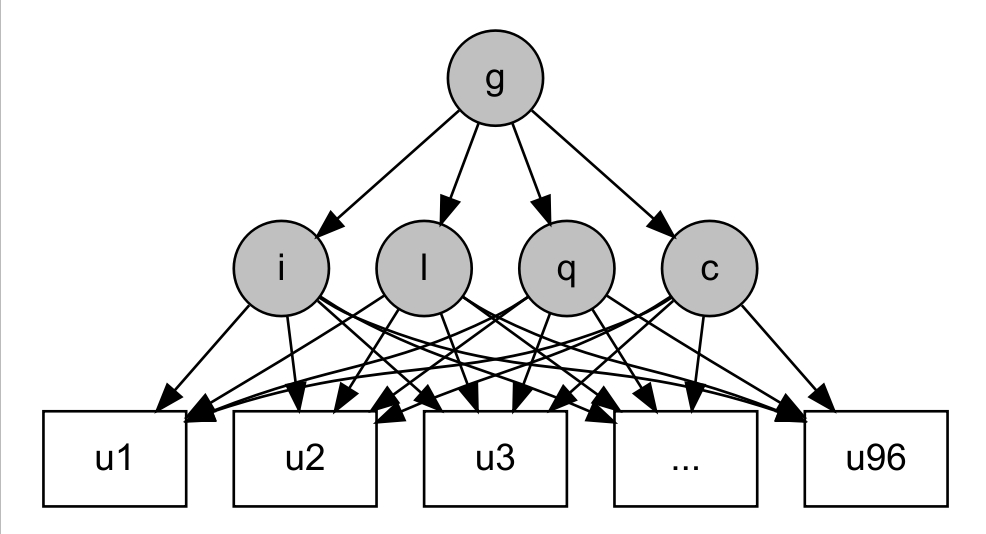
\includegraphics[width=10cm]{Figures/LCGAdiagramme.jpeg}
%	\decoRule
%	\caption[Diagramme for LCGA model]{Diagram for LCGA model.\\ \scriptsize{\textbf{Abbreviations:} g, latent class variable; i, intercept; l, linear term coefficient; q, quadratic term coefficient; c, cubic term coefficient; u1, u2, ... u96, repeated categorical outcomes of eating carbohydrates at each hour/time slots across four days of survey.}}
%	\label{fig:LCGAdiagram}
%\end{figure}\vspace{-0.6cm}
%
%In the NDNS RP data context, we considered a latent categorical variable $g_i$ representing the unobserved subpopulation membership (latent class variable) for participant $i, (g_{i} = 1,2,\cdots K)$. Then a LCGA model predicts the probability of the carbohydrate eating response $u_{ti}$ at time $t$ in latent class $K$ can be written as: \vspace{-0.3cm}
%
%\begin{equation}
%\begin{aligned}
%P(u_{ti} = 0/1/2 |g_i = K) &  = \frac{1}{1 + e^{-\text{logit}(u_{itK})}} \\
%\text{logit}(u_{itK}) & = \beta_{0K} + \beta_{1K}t_{i} + \beta_{2K}t^2_i + \beta_{3K}t^3_i + \epsilon_{i} \\ 
%\epsilon_{i} \sim N(0, \sigma^2) & \;i = 1,2,...6155
%\end{aligned}
%\end{equation}\vspace{-0.6cm}
%
%Where, 
%
%\begin{itemize}
%	\item $u_{ti}=\left\{ \begin{array}{ll}  0 & \text{if particiant } i \text{ was not eating any food at time } t\\ 
%	 1 & \text{if particiant } i \text{ was eating food and contribution of energy} \\ 
%	   &  \text{from carbohydrate was lower than 50\% at time } t \\ 
%	 2 & \text{if participant } i \text{ was eating food and contribution of energy} \\ 
%	 &  \text{from carbohydrate was higher or equal to 50\% at time } t \end{array} \right.$
%	\item $\beta_{0K}, \beta_{1K}, \beta_{2K}, \beta_{3K}$  correspond to $i, l, q, c$ in \textbf{Figure \ref{fig:LCGAdiagram}}, i.e. the coefficients for intercept, linear, quadratic, and cubic term of time.
%\end{itemize}
%
%An LCGA model can be modelled using either a linear, quadratic, or cubic trend over time. However, in our case, it may not be appropriate to assume the probabilities of responses to eating carbohydrates on the logit scale to change on a linear, or quadratic trend over four days, we chose to fit a more flex time function-a cubic form of time. The assumption in a LCGA model is that the data trajectory (the curve of eating carbohydrate pattern) for the participant consisting of the repeated measurements over time $t$, are independent given the group, $g_i$.



\subsection{Characteristics of day-level latent classes and individual-level latent classes}\vspace{-0.3cm}


Day-level latent classes identified by the first step of MLCA were tabulated according to the day of week and also whether the diary was recorded during weekends or not. A contingency table giving the frequency of responses across the 7-time slots of the survey days was produced. Descriptive statistics for the dietary day-level recordings according to the latent class memberships were presented. Pearson $\chi^2$ test was used to assess evidence fora difference in the distribution of categorical variables. One-way Analysis of Variance (ANOVA) was used to compare the means across the multiple groups for continuous variables.

Person-level point estimates and 95\% confidence intervals (CIs) were determined by applying individual, nurse visiting, and blood sample weights accordingly which account for the probability of participant selection and the clustered survey design. Descriptive statistics for sample characteristics were presented as weighted means (95\% CI) or weighted percentages (95\%CI). After examining the distribution of the data, the following variables were log-transformed to improve normality: fasting blood glucose, A1C, TC, LDL, HDL, TG, and average physical activity duration per day. Weighted geometric means (95\% CI) were used for all log-transformed variables. 

To see whether there is any temporal pattern for food intake eating could also be defined at the individual-level, weighted estimates of nutrients consumption across the 7-time slots of the day were calculated for each individual-level latent class. Contributions (\%) of the average energy intake within time slots were evaluated by determining the percentages of energy coming from carbohydrate, fat, protein, and alcohol intake. 

For continuous variables, the \textit{F} test was used to determine differences between latent classes with Bonferroni correction to account for multiple testing across $>$ 2 classes when applicable. For categorical variables, differences between latent classes were assessed using the adjusted Pearson $\chi^2$ test for survey data.\vspace{-0.5cm}


\subsection{Association between individual-level latent classes and the prevalence of hypertension, and measurements of obesity}\vspace{-0.3cm}


Associations between individual-level carbohydrate eating classes and hypertension (yes/no), body mass index (BMI, kg/m\textsuperscript{2}), and waist circumference (WC, cm) were explored in men and women separately. Point estimates of weighted means and proportions and 95\%CI of the characteristics were determined by applying either nurse visiting weights (for outcomes of hypertension, BMI, and WC) or blood sample weights (for diagnosis of DM) accordingly. Similarly, \textit{F} tests (for continuous variables) and adjusted Pearson $\chi^2$ tests (for categorical variables) were used to determine sex-specific differences by hypertension status, and BMI categories. 

%multinomial logistic regression model (for BMI categories),


Survey-designed logistic regression models (for hypertension), and linear regression models (for WC, BMI), were used to test for associations between latent classes of carbohydrate eating patterns and hypertension, BMI, and WC, in the NDNS RP sample, separately. Since diabetic participants might or might not modify their carbohydrate eating habits, we also fitted all the above-mentioned regression models restricted to those without diabetes.

For the multiple regression models, model fitting strategies are as follows: 

\begin{enumerate}
	\item The crude association between the carbohydrate eating groups and the outcomes was first examined. 
	\item Potential confounders of the association between carbohydrate eating groups (exposure) and the outcomes were selected depending on the descriptive statistical analyses conducted above, i.e. those associated with both the exposure and the outcome and also not on the causal pathway were selected as potential confounders. Covariates that are strongly related with the outcomes but not associate with carbohydrate eating groups may reduce the standard errors and improve the precisions, so they were also considered in the linear regression models. 
	\item Confounding and/or interaction effects from each of the potential factors were checked one by one. Interaction effects were tested using the adjusted Wald test for whether the regression coefficients of the interaction terms are simultaneously equal to zero.  
	\item A preliminary model that includes all of the variables suggested to be confounders in the previous step was established. 
	\item The remaining variables were added to the preliminary model one by one to see if any of them may be a confounder in the condition of the presence of the other covariates. 
	\item For logistic regression models (hypertension) under the survey data, goodness-of-fit was assessed using the adapted \code{svylogitgof} command in Stata \parencite{archer2006goodness}. Other diagnostics for regular logistic regression models, such as estimating the pseudo-R\textsuperscript{2},  AIC or BIC, checking the standardized Pearson residuals, or covariate pattern residuals are currently not available for weighted survey data. 
	\item For linear regression models (WC, BMI), the assumption of independent observations is violated as soon as we weight the sample. General checking such as QQ plots of the residuals (normality), plotting the residuals against fitted values (constant variance) are not available either. Outliers, leverage, and Cook's distance cannot be checked either, however, participants with extreme weightings (if any) were checked by removing them and refitting the models as a sensitivity analysis.
	\item Since under survey designed data, the sampling-weighted least squares are not maximum likelihood, it would not be possible to compare models using likelihood ratio test. Instead, adjusted Wald tests with $p < 0.05$ were used as criteria for variable inclusion in the final model. Another Stata command \code{linktest} was also used to  decide whether quadratic and cubic terms of continuous variables were necessary in improving fitting of the model \parencite{pregibon1980goodness}. 
\end{enumerate}

Data manipulation and preparation \textbf{(Appendix \ref{AppendixA})} were done in R version 3.5.1 \parencite{R3.5.1}. All statistical analyses, except for MLCA models, were performed with \code{svyset} command as implemented in Stata software version 15.1 \parencite{stata15}. The process of model fitting, covariate selection, and interaction effect testing for the association between carbohydrate eating patterns and hypertension is shown as an example in \textbf{Appendix \ref{AppendixD}}. All \textit{p} values were two-sided.
